% One LSTM cell. The cell state runs straight across the top.
\documentclass[tikz,border=2pt]{standalone}
% Shared preamble for the standalone TikZ figures of the talks.
%
% Every figure is a standalone .tex file in this folder, compiled to PDF with
% LuaLaTeX and included with \includegraphics at natural size, so its fonts
% match the slides (kpfonts-otf, as in the theme).
\usepackage{amsmath}
\usepackage{mathtools}
\usepackage{kpfonts-otf}
\usepackage{xcolor}
\usepackage{derivative}
\usepackage{tikz}
\usetikzlibrary{positioning,fit,arrows.meta,calc}

% Symbols used by the figures
\newcommand{\bm}[1]{\symbfit{#1}}
\newcommand{\Real}{\mathbb{R}}
\newcommand{\W}{\bm{w}}

% Node fills
\definecolor{nodeInput}{HTML}{EDEDED}
\definecolor{nodeOp}{HTML}{FBF6DE}
\definecolor{nodeOutput}{HTML}{E7F0FA}
\definecolor{nodeLayer}{HTML}{F1F1F1}
\definecolor{nodeGate}{HTML}{FBE9E7}
\definecolor{nodeState}{HTML}{E7F0FA}
\definecolor{backArrow}{HTML}{B03A2E}

\tikzset{
  edge/.style={-{Stealth[length=2.1mm]}, semithick},
  % computational graphs
  graphnode/.style={rectangle, draw=black!65, semithick, rounded corners=1.5pt,
    minimum height=8mm, minimum width=19mm, inner sep=3pt, align=center},
  inputnode/.style={graphnode, fill=nodeInput},
  opnode/.style={graphnode, fill=nodeOp},
  outputnode/.style={graphnode, fill=nodeOutput},
  % layer diagrams
  layernode/.style={graphnode, fill=nodeLayer, minimum width=13mm,
    minimum height=7.5mm},
  lossnode/.style={graphnode, fill=nodeOutput, minimum width=11mm,
    minimum height=7.5mm},
  backedge/.style={-{Stealth[length=2.1mm]}, semithick, draw=backArrow},
  elabel/.style={font=\footnotesize, inner sep=1.5pt},
  blabel/.style={font=\footnotesize, inner sep=1.5pt, text=backArrow},
  % recurrent cells
  gatenode/.style={rectangle, draw=black!65, semithick, rounded corners=1.5pt,
    fill=nodeGate, minimum height=7mm, minimum width=8mm, inner sep=2pt,
    font=\footnotesize},
  opcircle/.style={circle, draw=black!65, semithick, fill=white,
    inner sep=0pt, minimum size=5.2mm, font=\small},
  statenode/.style={graphnode, fill=nodeState, minimum width=11mm,
    minimum height=7mm},
}

\begin{document}
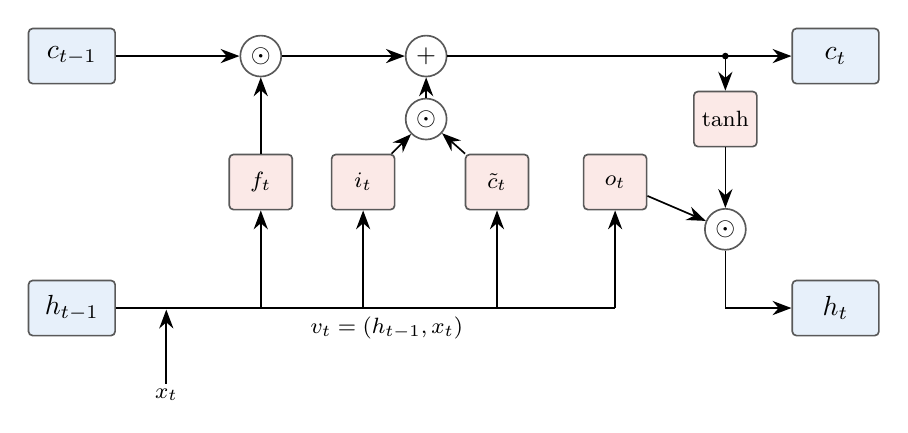
\begin{tikzpicture}[x=1cm, y=1cm, edge/.append style={-{Stealth[length=2.4mm]}}]
  % the cell state, straight across the top
  \node[statenode] (cprev) at (0,2.3) {$\bm c_{t-1}$};
  \node[opcircle]  (mulf)  at (2.4,2.3) {$\odot$};
  \node[opcircle]  (addc)  at (4.5,2.3) {$+$};
  \node[statenode] (cnext) at (9.7,2.3) {$\bm c_{t}$};
  \draw[edge] (cprev) -- (mulf);
  \draw[edge] (mulf) -- (addc);
  \draw[edge] (addc) -- (cnext);

  % gates and candidate
  \node[gatenode] (f)  at (2.4,0.7) {$\bm f_t$};
  \node[gatenode] (i)  at (3.7,0.7) {$\bm i_t$};
  \node[gatenode] (ct) at (5.4,0.7) {$\tilde{\bm c}_t$};
  \node[gatenode] (o)  at (6.9,0.7) {$\bm o_t$};
  \node[opcircle] (muli) at (4.5,1.5) {$\odot$};
  \node[gatenode] (th)   at (8.3,1.5) {$\tanh$};
  \node[opcircle] (mulo) at (8.3,0.1) {$\odot$};

  \draw[edge] (f) -- (mulf);
  \draw[edge] (i) -- (muli);
  \draw[edge] (ct) -- (muli);
  \draw[edge] (muli) -- (addc);
  \draw[edge] (8.3,2.3) -- (th);
  \fill (8.3,2.3) circle (1.2pt);
  \draw[edge] (th) -- (mulo);
  \draw[edge] (o) -- (mulo);

  % what the gates are computed from
  \node[statenode] (hprev) at (0,-0.9) {$\bm h_{t-1}$};
  \node[elabel] (x) at (1.2,-2.0) {$\bm x_t$};
  \node[statenode] (hnext) at (9.7,-0.9) {$\bm h_{t}$};
  \draw[semithick] (hprev) -- (6.9,-0.9);
  \draw[edge] (x) -- (1.2,-0.92);
  \node[elabel, below] at (4.0,-0.95) {$\bm v_t=(\bm h_{t-1},\bm x_t)$};
  \foreach \n in {f,i,ct,o}{\draw[edge] (\n|-hprev) -- (\n);}
  \draw[edge] (mulo) |- (hnext);
\end{tikzpicture}
\end{document}
